\documentclass[11pt]{article}

\usepackage[utf8]{inputenc}
\usepackage[T1]{fontenc}
\usepackage[english, french]{babel} %français
\usepackage[usenames,dvipsnames]{color} % color
\usepackage{amsmath}
\usepackage{amsfonts}
\usepackage{makeidx}
\usepackage{graphicx}
\usepackage[left=2cm,right=2cm,top=2cm,bottom=2cm]{geometry}
\usepackage{mathtools} %dcases
\usepackage{braket} %quantum mechanics
\usepackage[colorlinks=true, linkcolor=black, citecolor=black]{hyperref} % hyperlinks
\usepackage{tikz} % drawing in LaTeX

% subfigure
\usepackage{caption}
\usepackage{subcaption}

% the equal sign I use to define something
\newcommand{\define}{\ensuremath{ \overset{\text{def}}{=} }}

% differential element
\renewcommand{\d}[1]{\mathrm{d}#1}

% Hermitian conjugate
\DeclareMathOperator{\hc}{h.c.}

% Trace
\DeclareMathOperator{\tr}{tr}

% Equivalent sign in align environment
\newcommand{\eq}{\llap{$\Leftrightarrow$ \qquad}}

\title{\textbf{The hierarchical chain (tight binding model)}}
\author{}
\date{October 9, 2014}
\begin{document}

% I'm writing in english
\selectlanguage{english}

\maketitle

\section{The model}

\begin{center}
    	\begin{tikzpicture}[scale=1]
    		\newcommand{\orig}{-1.5}
    		\newcommand{\trans}{2}
    	
    		% bonds 
        	\draw[-] (\orig, 0) -- (\orig+\trans, 0) node [midway, above] {$t_0$};
			\draw[-,dashed] (\orig+\trans,0) -- (\orig+2*\trans,0) node [midway, above] {$t_1$};
			\draw[-] (\orig+2*\trans,0) -- (\orig+3*\trans,0) node [midway, above] {$t_0$};			
    	
    		% sites
			\filldraw (\orig,0) circle (0.05) node [below] {$\ket{0}$};
			\filldraw (\orig+\trans,0) circle (0.05) node [below] {$\ket{1}$};
			\filldraw (\orig+2*\trans,0) circle (0.05) node [below] {$\ket{2}$};
			\filldraw (\orig+3*\trans,0) circle (0.05) node [below] {$\ket{3}$};

		\end{tikzpicture}
\end{center}

We consider the tight-binding Hamiltonian:
\begin{equation}
	H = \sum_i t(i) \ket{i-1} \bra{i} + \hc
\end{equation}
where
\begin{equation}
	t(i) \define t_k\text{, with $k$ the number of times 2 divides $i$.}
\end{equation}
Such a Hamiltonian has a the structure of a binary tree. This binary hierarchy must somehow show up in its spectrum, at least given a reasonable set of $t_k$s.

\section{Strong hierarchy: $t_0 \gg t_1 \gg ... \gg t_1^2 \gg t_2^2 \gg ... \gg t_1^3 \gg t_2^3 \gg ...$}
In that case, we can treat the problem perturbatively ; first integrate out the diatomic molecules (two atoms liked by a $t_0$ bond), then the the diatomic molecules of diatomic molecules (two diatomic molecules linked by a $t_1$ bond), etc.

At the first order in perturbation theory the spectrum is
\begin{equation}
	E_{\epsilon_1\epsilon_2...} = (-1)^{\epsilon_1} t_0 + (-1)^{\epsilon_2} \frac{t_1}{2} + (-1)^{\epsilon_3} \frac{t_2}{4} + ...
\end{equation} 
At zeroth order in perturbation theory, the eigenstate assiated to $E_{\epsilon_1\epsilon_2...}$ can be constructed using the following procedure:
\begin{itemize}
	\item If $\epsilon_1 = 0/1$ construct the symmetric/antisymmetric linear combination of atomic states linked by a $t_0$ bond. That is to say, construct the vector
	\begin{equation}
		\ket{\psi^0_{\epsilon_1}} = \frac{1}{\sqrt{2}} ( \ket{0} + (-1)^{\epsilon_1} \ket{1} ) + \frac{1}{\sqrt{2}} ( \ket{2} + (-1)^{\epsilon_1} \ket{3} ) + ...
	\end{equation}
	We shall define $\ket{i,\epsilon_1} \define ( \ket{2i} + (-1)^{\epsilon_1} \ket{2i+1} )/\sqrt{2} $. We shall call the $\ket{i,\epsilon_1}$ the \emph{diatomic states}. If $\epsilon_1=0/1$ we say that the diatomic state $i$ is \emph{antibonding/bonding}.
	
	\item If $\epsilon_2 = 0/1$ construct the symmetric/antisymmetric linear combination of diatomic states linked by a $t_1$ bond. That is to say, construct the vector
	\begin{equation}
		\ket{\psi^1_{\epsilon_1 \epsilon_2}} = \frac{1}{\sqrt{2}} ( \ket{0,\epsilon_1} + (-1)^{\epsilon_2} \ket{1,\epsilon_1} ) + \frac{1}{\sqrt{2}} ( \ket{2,\epsilon_1} + (-1)^{\epsilon_2} \ket{3,\epsilon_1} ) + ...
	\end{equation}
	We shall define the \emph{quadriatomic states} $\ket{i,\epsilon_1 \epsilon_2} \define ( \ket{2i,\epsilon_1} + (-1)^{\epsilon_2} \ket{2i+1,\epsilon_1} )/\sqrt{2} $
	\item If $\epsilon_n = 0/1$ construct the symmetric/antisymmetric linear combination of $2^{n-1}$-atomic states linked by a $t_{n-1}$ bond.
\end{itemize}
At the $n^\text{th}$ step of this procedure, we obtain $\ket{\psi^{n-1}_{\epsilon_1...\epsilon_n}}$, the zeroth order eigenvector of a $2^n$ size hierarchical chain associated with the energy $E_{\epsilon_1...\epsilon_n}$.

\begin{figure}[htp]
\centering
  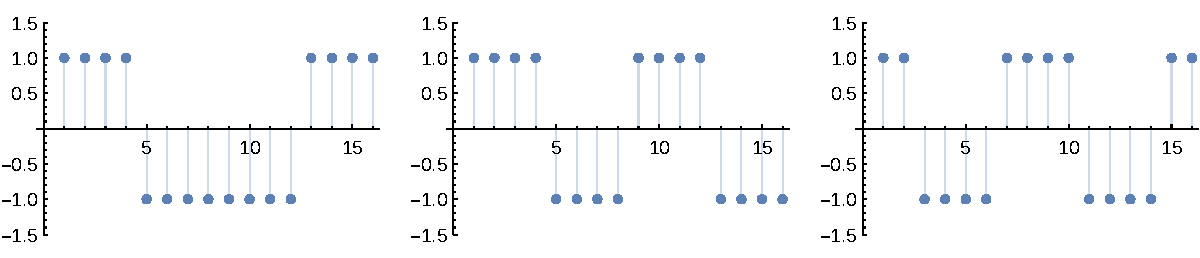
\includegraphics[width=.9\linewidth]{data/eigenfunctions_zeroth_order.pdf}
  \caption{From left to right: $2^4$-atomic states associated with the energies $\epsilon_1\epsilon_2\epsilon_3\epsilon_4 = 0010, 0011, 0100$, in the atomic states basis.}
  \label{fig:eigenfunctions_strong_hierarchy}
\end{figure}

\section{Geometric hierarchy: $t_{k\geq2} = R t_{k-1}$}
In that case, we may no longer be able to organize the perturbation theory hierarchically (for example second order perturbation theory applied to the $2^2$ chain will involve corrections of order $t_2^2 = R^2 t_1^2$, but since $t_3 = R^2 t_1 = t_2^2/t_1$, depending on the value of $t_1$, these second order corrections may be involved when dealing with the $2^{3}$ chain at first order.).

Following \cite{transitionmatrix}, we chose
\begin{equation}
t_k = \begin{dcases*}
        1  & if $k=0$ \\
        V & if $k=1$\\
        R^{k-2} V & if $k > 1$
        \end{dcases*}
\end{equation}

\subsection{Spectrum and wavefunctions}


\begin{figure}[htp]
\centering
\begin{subfigure}{.5\textwidth}
  \centering
  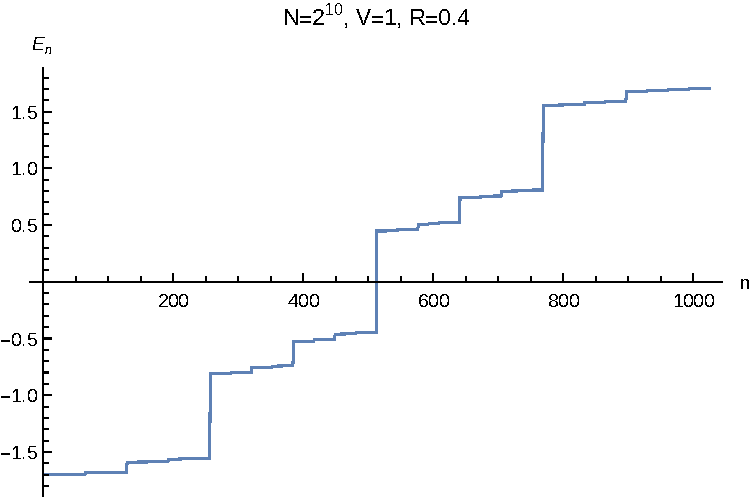
\includegraphics[width=.9\linewidth]{data/spectrum_isolated_hchain.pdf}
  \caption{Spectrum of the isolated chain of $N$ atomic sites.}
  \label{fig:sp_isolated}
\end{subfigure}%
\begin{subfigure}{.5\textwidth}
  \centering
  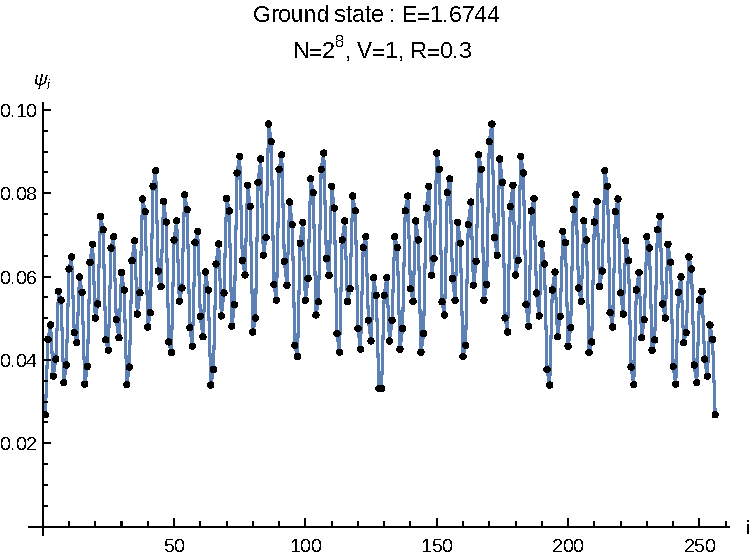
\includegraphics[width=.9\linewidth]{data/ground_state_isolated_hchain.pdf}
  \caption{Ground state of the chain of $N$ atomic sites.}
  \label{fig:gs_isolated}
\end{subfigure}
\caption{Numerical results for the isolated chain with geometric hierarchy.}
\label{fig:num_geom}
\end{figure}

As before, we consider an isolated chain of $N=2^n$ atoms.

\begin{center}
    	\begin{tikzpicture}[scale=1]
    		\newcommand{\orig}{-1.5}
    		\newcommand{\trans}{2}
    	
    		% bonds 
        	\draw[-] (\orig, 0) -- (\orig+\trans, 0) node [midway, above] {$1$};
			\draw[-,dashed] (\orig+\trans,0) -- (\orig+2*\trans,0) node [midway, above] {$V$};
			\draw[-] (\orig+2*\trans,0) -- (\orig+3*\trans,0) node [midway, above] {$1$};
			\draw[-,dotted] (\orig+3*\trans,0) -- (\orig+4*\trans,0) node [midway, above] {$RV$};
			\draw[-] (\orig+4*\trans,0) -- (\orig+5*\trans,0) node [midway, above] {$1$};
			\draw[-,dashed] (\orig+5*\trans,0) -- (\orig+6*\trans,0) node [midway, above] {$V$};
			\draw[-] (\orig+6*\trans,0) -- (\orig+7*\trans,0) node [midway, above] {$1$};
    	
    		% sites
			\filldraw (\orig,0) circle (0.05) node [below] {$\ket{0}$};
			\filldraw (\orig+\trans,0) circle (0.05) node [below] {$\ket{1}$};
			\filldraw (\orig+2*\trans,0) circle (0.05) node [below] {$\ket{2}$};
			\filldraw (\orig+3*\trans,0) circle (0.05) node [below] {$\ket{3}$};
			\filldraw (\orig+4*\trans,0) circle (0.05) node [below] {$\ket{4}$};
			\filldraw (\orig+5*\trans,0) circle (0.05) node [below] {$\ket{5}$};
			\filldraw (\orig+6*\trans,0) circle (0.05) node [below] {$\ket{6}$};
			\filldraw (\orig+7*\trans,0) circle (0.05) node [below] {$\ket{7}$};

		\end{tikzpicture}
\end{center}

Numerically, we can easily compute its spectrum (fig. \eqref{fig:sp_isolated}) and the corresponding wavefunctions (fig. \eqref{fig:gs_isolated}). It looks like both spectrum and wavefunctions have a hierarchical structure.

To further analize the hierarchical character of the spectrum, we wish to compute its fractal dimensions (aka Rényi dimensions or Rényi entropy or generalized dimensions)

\subsection{Fractal dimensions}

We consider our spectrum as a subset of some set (say the unit interval $I=[0,1]$), that we partition into boxes of length $\epsilon$. 
Following \cite{Halsey1986} we then define $p_i$ as the fraction of points of our spectrum lying inside the $i^\text{th}$ box. The $q^\text{th}$ generalized/fractal/Rényi dimension is then 
\begin{equation}
	D_q = \frac{1}{q-1}\lim_{\epsilon \rightarrow 0} \frac{\log \sum_i p_i^q}{\log \epsilon^{-1}}
\end{equation}

\subsubsection{Box-counted Hausdorff dimension}

We have
\begin{equation}
	D_0 = - \lim_{\epsilon \rightarrow 0} \frac{\log N_b}{\log \epsilon^{-1}}
\end{equation}
where $N_b$ is the number of boxes containing at least one point of the spectrum.
This is the reason why $D_0$ is called the \emph{box-counting} dimension.
In most cases the Hausdorff dimension coincides with the box-counting dimension\footnote{In fact $D_0$ is always greater or equal to the Hausdorff dimension. Indeed, countable sets increase the dimension $D_0$ -- obtained by box-counting -- when they have accumulation points, while they do not contribute to the Hausdorff dimension.}. 

\begin{figure}[htp]
\centering
\begin{subfigure}{.5\textwidth}
  \centering
  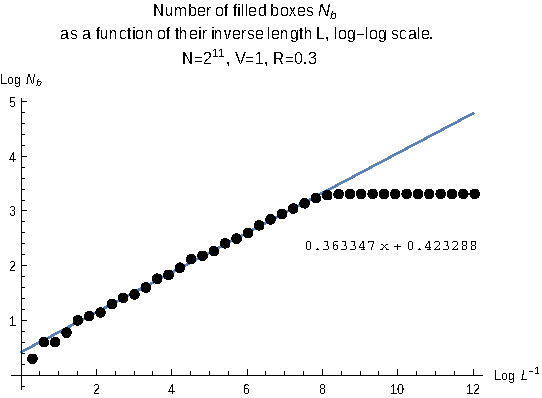
\includegraphics[width=.9\linewidth]{data/box_counting.pdf}
  \caption{$D_0$ obtained by direct box-counting.}
  \label{fig:direct_bc}
\end{subfigure}%
\begin{subfigure}{.5\textwidth}
  \centering
  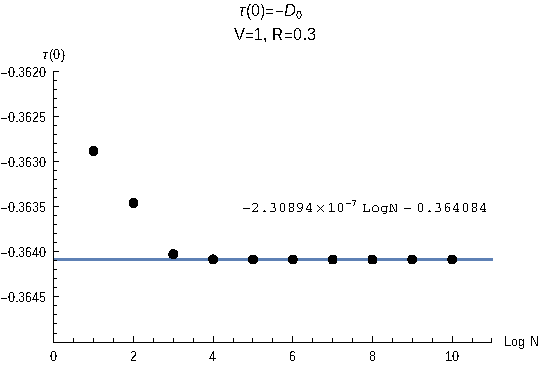
\includegraphics[width=.9\linewidth]{data/hausdorff.pdf}
  \caption{$D_0$ obtained with the partition function.}
  \label{fig:partition_bc}
\end{subfigure}
\caption{Box-counting.}
\label{fig:bc}
\end{figure}

Figure \eqref{fig:direct_bc} shows how $\log N_b$ evolve as $\epsilon \rightarrow 0$, in $\log-\log$ scale. 
For an infinite size system (that is, for the spectrum of the infinite chain) we expect this function to have a linear asymptotic behaviour, the slope of the asymptote being $-D_0$.
For our numerical, finite size spectrum however, we expect finite size effects to come into play when $\epsilon$ is too small.
This is indeed what happens (fig. \eqref{fig:direct_bc}). For this computation we took a sequence of boxes of length $\epsilon_i = \delta^{-i}$. We noted that when $\delta$ is taken to be a power of 2, $\log N_b$ becomes constant when $\epsilon$ is sufficiently small (in fig. \eqref{fig:direct_bc} $\delta$ was set to 2). Whereas when $\delta$ is not a power of 2, $\log N_b$ seems to be taking random values when $\epsilon$ is sufficiently small. 
This probably means that the energy states are indexed by a binary integer, at least for finite size chains.

\subsubsection{Partition function}

The \emph{partition function} $\Gamma$ is another tool one can use to compute the fractal dimensions. 

Let us consider a partition $\mathcal{P}=\{ S_i \}_i$ of the set $S$ whose fractal dimensions we are interested in. Each subset $S_i$ is contained in a ball of radius $l_i$. This ball contains a fraction $p_i$ of the points of $S$. 
We assume that the balls radii are smaller than a control radius $\epsilon$.
Then we define the \emph{partition function}:
\begin{equation}
	\Gamma(q,\tau;\mathcal{P}, \{l_i\}) \define \sum_i \frac{p_i^q}{l_i^\tau}
\end{equation}
Next, we chose the partition such as to minimize/maximize $\Gamma$ depending on whether $q$ is positive/negative:
\begin{equation}
\Gamma(q,\tau) \define \begin{dcases*}
        \inf_{\mathcal{P}} \Gamma(q,\tau;\mathcal{P}, \{l_i\}) & if $q>0$ \\
        \max_{\mathcal{P}} \Gamma(q,\tau;\mathcal{P}, \{l_i\}) & if $q<0$
        \end{dcases*}
\end{equation}
It is not clear for me at the moment how we chose the radii $l_i$.
In the limit $\epsilon \rightarrow 0$, the above partition function is finite only when $\tau \define \tau(q)$. We have the important property
\begin{equation}
	\tau(q) = (q-1) D_q
\end{equation}

\begin{figure}[htp]
\centering
  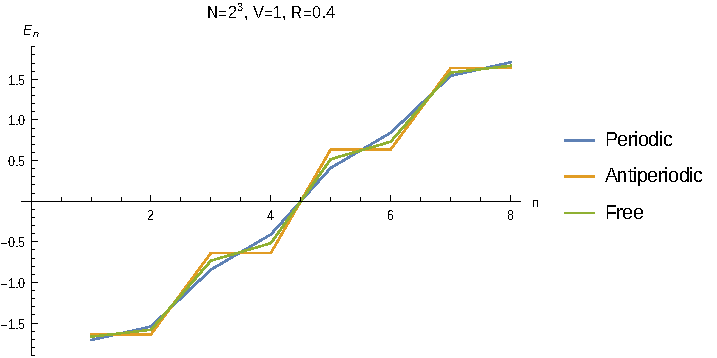
\includegraphics[width=.8\linewidth]{data/spectra_vs_bc_hchain.pdf}
  \caption{Spectrum of the chain with $2^3$ sites for different boundary conditions.}
  \label{fig:spectra_bc}
\end{figure}

In our case, the set $S$ is the spectrum of the infinite chain. 
We can compute a sequence of spectra $\{S^p_n\}_n, \{S^a_n\}_n$, $S^p_n$ and $S^a_n$ being the spectrum of the chain of length $2^n$ with periodic/antiperiodic boundary conditions. In the limit $n\rightarrow \infty$ both spectra become equal to $S$.
If we wish to compute $\Gamma_n(q,\tau)$, the $n^\text{th}$ approximant of the partition function, we must find a suitable partition $\mathcal{P}_n$ and a suitable associated set of radii $l_i$.
As the spectra $S^p_n, S^a_n$ are finite sets, it seems natural to partition them into insolated points. To each point we must now associate a ball of radius $l_i$. What should we take as a radius ? I don't know why, but it turns out to be a great idea to chose $l_i$ to be the distance betweeen a point $S^p_n$ and the corresponding point of $S^a_n$. 
The chain of length $2^n$ with any boundary condition has energies sandwiched between the associated energy for the periodic boundary conditions and the associated energy for antiperiodic boundary conditions (fig \eqref{fig:spectra_bc}). Thus, we understand that $\Gamma_n(q,\tau;\mathcal{P},\{l_i\})$ is a good candidate for the partition function of the spectrum of the chain of length $2^n$ with any boundary condition
Of course $p_i = 2^{-n}$ as the $2^n$ sites chain has $2^n$ (nondegenerate) energies.

To evaluate numerically $\tau(q)$ we can either find $\tau$ such that $\Gamma_{n\rightarrow \infty}$ is finite, or find $\tau$ such that 
\begin{equation}
	\lim_{n\rightarrow \infty} \frac{\Gamma_{n+1}}{\Gamma_n} = 1
\end{equation}
The latter method seems more accurate. We solved $\Gamma_{n+1}/\Gamma_n = 1$ for increasing values of $n$. The result is fig \eqref{fig:partition_bc}. The convergence seems to be quite quick. 
The Hausdorff dimension obtained with this method agrees with the one obtained by direct box-counting up to the third decimal place.

\subsection{Transition matrices}

\subsubsection{Definition}
For a nearest-neighbours tight-binding system, the Schrödinger equation writes
\begin{equation}
	E \psi_n = t_{n,n-1} \psi_{n-1} + t_{n,n+1} \psi_{n+1}
\end{equation}
where $\psi_n = \braket{n|\psi}$. In the hierarchical chain case, the hopping amplitudes are real-valued: $t_{n,n+1} = t_{n+1,n}^* = t_{n+1,n} \define t(n)$.

In general, we can define a \emph{transition matrix}:
\begin{equation}
	T(t_r,t_l;E) \define 
	\begin{bmatrix}
		\frac{E}{t_r} & -\frac{t_l}{t_r}\\
		1 & 0\\
	\end{bmatrix}
\end{equation}
and we have the important property that
\begin{equation}
	\underbrace{T(t_{n,n+1},t_{n,n-1};E)}_{ \define T_{n,n-1} } 
	\begin{pmatrix}
		\psi_n\\
		\psi_{n-1}\\
	\end{pmatrix}
	= 
	\begin{pmatrix}
		\psi_{n+1}\\
		\psi_{n}\\
	\end{pmatrix}
\end{equation}

\subsubsection{Application to the (periodic) hierarchical chain}

\begin{figure}[htp]
\centering
    	\begin{tikzpicture}[scale=1]
    		\newcommand{\orig}{-1.5}
    		\newcommand{\trans}{2}
    	
    		% bonds 
        	\draw[-] (\orig, 0) -- (\orig+\trans, 0) node [midway, above] {$1$};
			\draw[-,dashed] (\orig+\trans,0) -- (\orig+2*\trans,0) node [midway, above] {$V$};
			\draw[-] (\orig+2*\trans,0) -- (\orig+3*\trans,0) node [midway, above] {$1$};
			\draw[-,dashed] (\orig+3*\trans,0) -- (\orig+4*\trans,0) node [midway, above] {$V$};
    	
    		% sites
			\filldraw (\orig,0) circle (0.05) node [below] {$\ket{0}$};
			\filldraw (\orig+\trans,0) circle (0.05) node [below] {$\ket{1}$};
			\filldraw (\orig+2*\trans,0) circle (0.05) node [below] {$\ket{2}$};
			\filldraw (\orig+3*\trans,0) circle (0.05) node [below] {$\ket{3}$};
			\filldraw (\orig+4*\trans,0) circle (0.05) node [below] {$\ket{4}$};
		\end{tikzpicture}
	\caption{First periodic approximant of the hierarchical chain. Two periods are shown.}
\end{figure}

We now consider the $n^\text{th}$ periodic approximant of the infinite hierarchical chain. It is defined as the infinite chain obtained by the replacement
\begin{equation}
	t_{k > n} \rightarrow t_{n}
\end{equation}
The $n^\text{th}$ periodic approximant has period $2^n$.

\textbf{First periodic approximant:} because the first periodic approximant has period $2$, we have
\begin{equation}
	T(1,V;E)T(V,1;E)
	\begin{pmatrix}
		\psi_1\\
		\psi_{0}\\
	\end{pmatrix} = T_{2,1}T_{1,0}
	\begin{pmatrix}
		\psi_1\\
		\psi_{0}\\
	\end{pmatrix} = 
	\begin{pmatrix}
		\psi_3\\
		\psi_{2}\\
	\end{pmatrix}
	= e^{2ik} 
	\begin{pmatrix}
		\psi_1\\
		\psi_{0}\\
	\end{pmatrix}
\end{equation}
We see that the vector $(\psi_1,\psi_0)$ is an eigenvector of $T_{2,1} T_{1,0}$, associated to the eigenvalue $\lambda_1 = \exp(2ik)$.
Moreover, because of the periodicity,
\begin{equation}
	\det T_{2,1}T_{1,0} = 1
\end{equation}
So that $\lambda_1 \lambda_2 = 1$. Thus $\lambda_2 = \lambda_1^* = \exp(-2ik)$, and
\begin{equation}
	\tr T_{2,1}T_{1,0} = \frac{E^2-V^2-1}{V} = 2 \cos(2 k)
\end{equation}
Solving this second-order polynomial in $E$ gives us the two energy bands of this first periodic approximant.

\textbf{Second periodic approximant and decimation:}
\begin{figure}[htp]
\centering
    	\begin{tikzpicture}[scale=1]
    		\newcommand{\orig}{-1.5}
    		\newcommand{\trans}{2}
    	
    		% bonds 
    		\draw[-,dotted,red] (\orig-\trans,0) -- (\orig,0) node [midway, above] {$RV$};
        	\draw[-] (\orig, 0) -- (\orig+\trans, 0) node [midway, above] {$1$};
			\draw[-,dashed] (\orig+\trans,0) -- (\orig+2*\trans,0) node [midway, above] {$V$};
			\draw[-] (\orig+2*\trans,0) -- (\orig+3*\trans,0) node [midway, above] {$1$};
			\draw[-,dotted] (\orig+3*\trans,0) -- (\orig+4*\trans,0) node [midway, above] {$RV$};

    		% sites
    		\filldraw [red] (\orig-\trans,0) circle (0.05) node [below] {$\ket{-1}$};
			\filldraw (\orig,0) circle (0.05) node [below] {$\ket{0}$};
			\filldraw (\orig+\trans,0) circle (0.05) node [below] {$\ket{1}$};
			\filldraw (\orig+2*\trans,0) circle (0.05) node [below] {$\ket{2}$};
			\filldraw (\orig+3*\trans,0) circle (0.05) node [below] {$\ket{3}$};
			\filldraw [red] (\orig+4*\trans,0) circle (0.05) node [below] {$\ket{4}$};
		\end{tikzpicture}
	\caption{Second periodic approximant. One period is shown (in black), as well as the surrounding environment (in red).}
	\label{fig:decim_2}
\end{figure}
For this second periodic approximant, the period is $2^2=4$. We do not wish to compute directly the 4 bands, but rather to decimate half the sites of this period 4 system in order to recover a system equivalent to the previously studied period 2 system.

\begin{figure}[htp]
\centering
    	\begin{tikzpicture}[scale=1]
    		\newcommand{\orig}{-1.5}
    		\newcommand{\trans}{2}
    	
    		% bonds 
    		\draw[-,dashed,red] (\orig-\trans,0) -- (\orig,0) node [midway, above] {$V'$};
        	\draw[-] (\orig, 0) -- (\orig+\trans, 0) node [midway, above] {$1$};
			\draw[-,dashed] (\orig+\trans,0) -- (\orig+2*\trans,0) node [midway, above] {$V'$};

    		% sites
    		\filldraw [red] (\orig-\trans,0) circle (0.05) node [below] {$\ket{-1'}$};
			\filldraw (\orig,0) circle (0.05) node [below] {$\ket{0'}$};
			\filldraw (\orig+\trans,0) circle (0.05) node [below] {$\ket{1'}$};
			\filldraw [red] (\orig+2*\trans,0) circle (0.05) node [below] {$\ket{2'}$};
		\end{tikzpicture}
	\caption{First periodic approximant with renormalized couplings.}
	\label{fig:decim_1}
\end{figure}

We chose to decimate the two sites surrounding the $V$ coupling (sites $\ket{1}$ and $\ket{2}$ in fig \eqref{fig:decim_2}). We will thus obtain a first periodic approximant with renormalized couplings (fig \eqref{fig:decim_1}).

Using transition matrices, this means that we wish to make the identification
\begin{align}
	T(RV,1;E)T(1,V;E)T(V,1;E)T(1,RV;E) &= T(V',1;E')T(1,V';E') \\
	\eq T_{3,2}T_{2,1}T_{1,0}T_{0,-1} &= T'_{1',0'}T'_{0',-1'} \\
	\eq \begin{bmatrix}
			\frac{(E^2-1)^2-E^2V^2}{RV^2} & -\frac{E}{V}(E^2-V^2-1)\\
			\frac{E}{V}(E^2-V^2-1) & -R(E^2-V^2)\\
		\end{bmatrix} &=
		\begin{bmatrix}
			\frac{E^{\prime2}-1}{V'} & -E'\\
			E' & -V'\\
		\end{bmatrix}
\end{align}
And thus, we conclude that the second approximant reduces to the first with the renormalized couplings
\begin{equation}
	\begin{dcases*}
        	V' &= $R(E^2-V^2)$ \\
        	E' &= $\frac{E}{V}(E^2-V^2-1)$
     \end{dcases*}
\end{equation}

\textbf{$n^\text{th}$ periodic approximant and decimation:}
We now wish to extend this decimation procedure to an arbitrary long approximant. 
This is easily done, because
\begin{equation}
	T({R^{\color{red}2}}V,1;E)T(1,V;E)T(V,1;E)T(1,RV;E) = T({\color{red}R}V',1;E')T(1,V';E')
\end{equation}
and
\begin{equation}
	T(RV,1;E)T(1,V;E)T(V,1;E)T(1,{R^{\color{red}2}}V;E) = T(V',1;E')T(1,{\color{red}R}V';E')
\end{equation}
with the same renormalized couplings $E'$ and $V'$.
The $n^\text{th}$ periodic approximant with couplings $E_n$ and $V_n$ thus reduces to the $(n-1)^\text{th}$ one with the renormalized couplings
\begin{equation}
	\begin{dcases*}
        	V_{n-1} &= $R(E_n^2-V_n^2)$ \\
        	E_{n-1} &= $\frac{E_n}{V_n}(E_n^2-V_n^2-1)$
     \end{dcases*}
\end{equation}
\bibliography{bib/hierarchical_chain_tight_binding.bib}{}
\bibliographystyle{plain}
\end{document}
